% default values
\def\ttau{1} % Zeitkonstante tau

% Plot Umgebung:
\def\samples{41}

\def\xomegaordermin{-2}
\def\xomegaordermax{2}
\def\xomegamin{1e\xomegaordermin}
\def\xomegamax{1e\xomegaordermax}

\def\yamptiefmin{0.8*1/(1+(\xomegamax*\ttau)^2)^0.5}
\def\yamptiefmax{2}

\def\yamphochmin{0.6e-2}
\def\yamphochmax{2}

\def\yphitiefmax{+10}
\def\yphitiefmin{-100}
\def\yphitiefg{-45}

\def\yphihochmin{-10}
\def\yphihochmax{100}
\def\yphihochg{45}

%%%%%%%%%%%%%%%%%%%%%%%%%%%%%%%%%%%%%%%%%%%%%%%%%%%%%%%%%%%%%%%%%%%%%%%%%%%%

% RC-Tiefpass 1. Ord. Amplitudengang
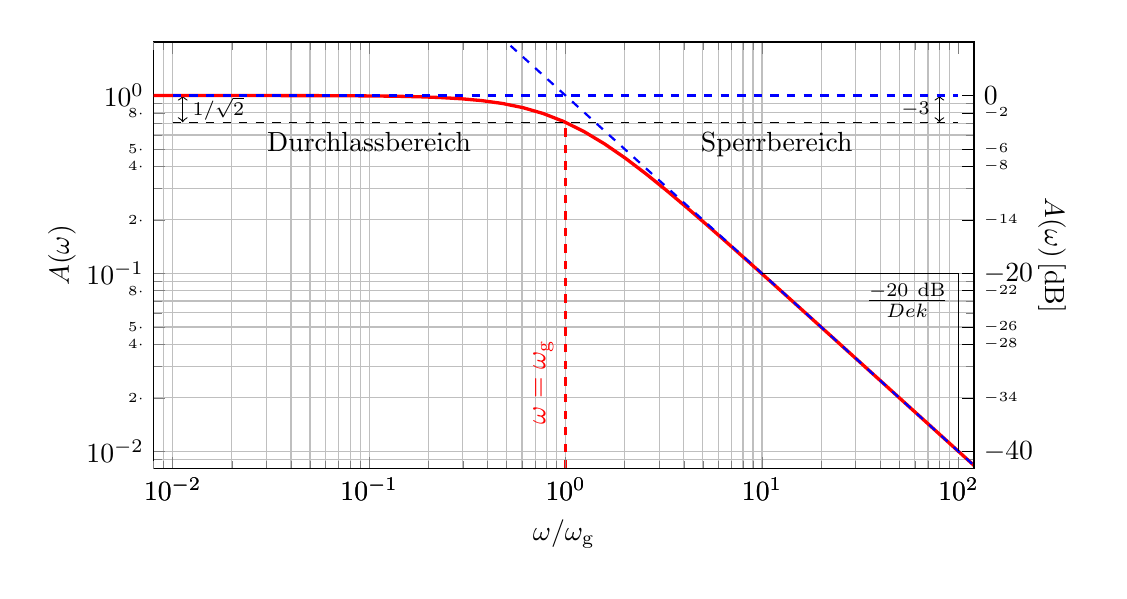
\begin{tikzpicture}[x=1mm,y=1mm] % gilt für tikz-coordinaten außerhalb der axis-environment
    \draw[draw=none] (-16,-13) rectangle (120,56); % Bildrahmen, Koordinatenbezug auf (0,0) des \begin{axis}...\end{axis} pgfplots, für
    \begin{axis}[
        %title={Amplitudengang RC-Tiefpass 1. Ordnung},
        xmode=log,ymode=log,
        xlabel={$\omega/\omega_{\mathrm{g}}$},
        ylabel={$A(\omega)$},
        ylabel shift = -3 pt,
        xmin=0.8*\xomegamin, xmax=1.2*\xomegamax,
        ymin=\yamptiefmin, % 0.8*0.01 (manual cut off bottom)
        ymax=\yamptiefmax,
        domain=0.8*\xomegamin:1.2*\xomegamax,
        samples=\samples,
        width=12cm,
        height=7cm,
        grid=minor,
        mark=none,
        extra y ticks={
            0.02, 0.04, 0.05, 0.08,
            0.20, 0.40, 0.50, 0.80
        },%0.7071
        extra y tick labels={
            $\scriptscriptstyle2\cdot$,$\scriptscriptstyle4\cdot$,$\scriptscriptstyle5\cdot$,$\scriptscriptstyle8\cdot$,
            $\scriptscriptstyle2\cdot$,$\scriptscriptstyle4\cdot$,$\scriptscriptstyle5\cdot$,$\scriptscriptstyle8\cdot$
        },%$\scriptscriptstyle-3$
    ]   
        % -3dB Grenze
        \addplot[black,<->] coordinates {(1.125*\xomegamin,1) (1.125*\xomegamin,0.7071)}node[pos=0.5,right]{$\scriptstyle{1/\sqrt{2}}$}; % Abstand -3dB
        \addplot[black,<->] coordinates {(0.800*\xomegamax,1) (0.800*\xomegamax,0.7071)}node[pos=0.5,left]{$\scriptstyle{-3\dB}$};       % Abstand -3dB
        \addplot[draw=none] coordinates {(\xomegamin,0.707) (1.000,0.707)} node[pos=0.50,below]{Durchlassbereich}; % Bereich
        \addplot[draw=none] coordinates {(\xomegamax,0.707) (1.414,0.707)} node[pos=0.5,below]{Sperrbereich};      % Bereich
        
        % Plot A(w/w0) = 1/sqrt(1+(w/w0)^2)
        \addplot[very thick,red,]   {1/(1+(x)^2)^ 0.5};
        
        % Näherungen, Hilfslinien
        \addplot[dashed,black,]  coordinates { (\xomegamin, 1/2^0.5) ( \xomegamax, 1/2^0.5) }; % Grenze -3dB
        \addplot[dashed,thick,blue] coordinates { (\xomegamin,1) (\xomegamax,1) };% Asymptote
        \addplot[dashed,thick,blue] {1/(x)};% Asymptote
        \draw (1e1,1e-1) -| (1e2,1e-2) node[pos=0.5,anchor=north east]{$\frac{-20\ \mathrm{dB}}{Dek}$}; %  -20dB/Dek (static)
        \addplot[dashed,thick,red] coordinates { (1/(\ttau),\yamptiefmin) (1/(\ttau),1/2^0.5)} 
            node [pos=0.25,sloped,style={yshift=8pt}] {$\omega=\omega_{\mathrm{g}}$};% % omega = omega_0

    \end{axis}
    \begin{axis}[
        xmode=log,ymode=log,
        axis y line*=right,                             % ylabel right
        ylabel={$A(\omega) \left[\mathrm{dB}\right]$},% ylabel right
        ylabel shift = -5 pt,
        ylabel style={rotate=180},
        xmin=0.8*\xomegamin, xmax=1.2*\xomegamax,
        ymin= 0.8 * 1/(1+(\xomegamax*\ttau)^2)^0.5,
        ymax=\yamptiefmax,
        width=12cm,
        height=7cm,
        grid=none,%grid=minor,
        ytick={0.01,0.1,1},
        yminorticks=false,
        ytick style={draw=black},
        yticklabels={$-40$,$-20$,$0$},
        extra y ticks={0.02,0.04,0.05,0.08,0.2,0.4,0.5,0.8},%0.7071
        extra y tick labels={$\scriptscriptstyle-34$,$\scriptscriptstyle-28$,$\scriptscriptstyle-26$,$\scriptscriptstyle-22$,$\scriptscriptstyle-14$,$\scriptscriptstyle-8$,$\scriptscriptstyle-6$,$\scriptscriptstyle-2$},%$\scriptscriptstyle-3$
    ]        
    \end{axis}
\end{tikzpicture}%